\documentclass[whitelogo]{tudelft-report}

% Packages
\usepackage{natbib}
\usepackage{changes}
\usepackage{inputenc}
\usepackage{float}
\usepackage{graphicx}
\usepackage[justification=centering]{caption}





\begin{document}

%% Use Roman numerals for the page numbers of the title pages and table of
%% contents.
\frontmatter

%% Uncomment following 19 lines for a cover with a picture on the lower half only
% \title[tudelft-white]{Title}
% \subtitle[tudelft-cyan]{Optional subtitle}
% \author[tudelft-white]{J.\ Random Author}
% \affiliation{Technische Universiteit Delft}
% \coverimage{cover.jpg}
% \titleoffsetx{10cm}
% \titleoffsety{10cm}
% \afiloffsetx{1cm}
% \afiloffsety{18cm}
% \covertext[tudelft-white]{
%     \textbf{Cover Text} \\
%     possibly \\
%     spanning 
%     multiple 
%     lines
%     \vfill
%     ISBN 000-00-0000-000-0
% }
% \makecover

%% Uncomment following 16 lines for a cover with a picture on the lower half only
\title[tudelft-white]{Title}
\subtitle[tudelft-black]{Optional subtitle}
\author[tudelft-white]{author1}
\affiliation{Technische Universiteit Delft}
\coverimage{tank.jpg}
\covertext[tudelft-white]{
    \textbf{Cover Text} \\
    possibly \\
    spanning 
    multiple 
    lines
    \vfill
    ISBN 000-00-0000-000-0
}
\setpagecolor{tudelft-cyan}
\makecover[split]


%% Include an optional title page.
\begin{titlepage}


\begin{center}

%% Print the title in cyan.
{\makeatletter
\largetitlestyle\fontsize{44}{48}\selectfont\@title
%\largetitlestyle\color{tudelft-cyan}\Huge\@title
\makeatother}

\vspace{1cm}

%% Print the optional subtitle in black.
{\makeatletter
\ifx\@subtitle\undefined\else
    \bigskip
   {\tudsffamily\fontsize{24}{28}\selectfont\@subtitle}    
    %\titlefont\titleshape\LARGE\@subtitle
\fi
\makeatother}

\bigskip
\bigskip
% hier je afbeelding voor de voorkant
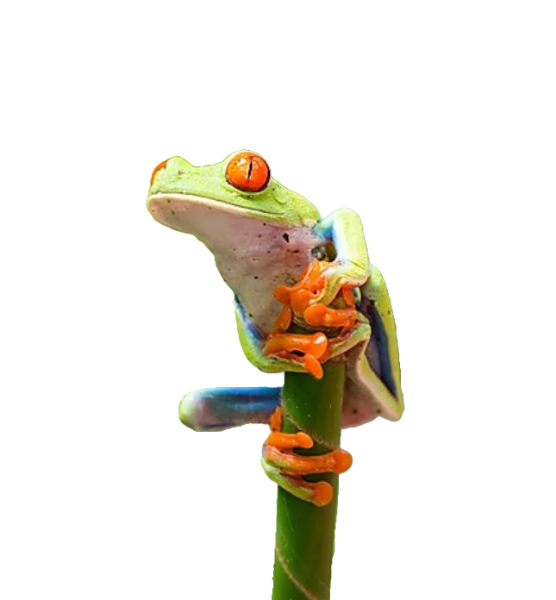
\includegraphics[width=0.75\linewidth]{images/kikker_voorkant.png}
\bigskip
\bigskip

%% Print the name of the author.
{\makeatletter
%\largetitlefont\Large\bfseries\@author
\largetitlestyle\fontsize{26}{26}\selectfont\@author
\makeatother}

\vspace{1cm}

\fontsize{15}{15} \tudsffamily \today

\vfill

\begin{table}[H]
    \Large
    \centering
    \begin{tabular}{l|l}
    R. Copier & 4354095
    \end{tabular}
\end{table}




%\centering{
\includegraphics{cover/logo_black}}


\end{center}

\begin{tikzpicture}[remember picture, overlay]
    \node at (current page.south)[anchor=south,inner sep=0pt]{
        
\includegraphics{cover/logo_black}
    };
\end{tikzpicture}


\end{titlepage}


\tableofcontents

\input{chapters/summary.tex}

%% Use Arabic numerals for the page numbers of the chapters.
\mainmatter

\input{chapters/userRequirements.tex}
\input{chapters/systemdescription.tex}
\input{chapters/OBS.tex}
\input{chapters/WFD.tex}
\input{chapters/WBS.tex}
\input{chapters/Designschedule.tex}
\input{chapters/PLD.tex}
\input{chapters/rules.tex}
\input{chapters/approach.tex}

%\input{appendix-a}
\bibliography{report}


%% Use letters for the chapter numbers of the appendices.
\appendix

\end{document}

